% 第4章 设计

% URN的目标是实现一个统一的软件虚拟化架构,能够同时为虚拟机和容器提供RDMA服务,并实现对虚拟RDMA的统一管理。此外,该框架还需具备与原生RDMA接近的高性能。在本章,介绍了URN中的一些关键性设计工作。
% The goals of URN is to achieve a unified RDMA virtualization framework for both containers and VMs. In this framework, virtual RDMA network are managed centrally. Besides, performance are also should be made close to native RDMA. In this section, we introduce some key designs for above goals.

% 4.1 vRNIC Design:

% vRNIC是一个软件的虚拟RDMA设备,包含前后端,前端负责为上层verb库提供接口并转发RDMA 命令,后端在主机端,通过与URN core或verbs库交互,以模拟guest对vRNIC的RDMA操作。 vRNIC继承了控制和数据通道分离的RDMA虚拟化工作,例如hyv和MasQ,控制路径上guest应用在本地的虚假RDMA上下文中执行verbs命令,并经过FE转发到BE维持的真实RDMA上下文中执行,之后将结果返回给guest;在数据路径上,将guest应用的RDMA资源与vRNIC BE上下文中的RDMA资源进行映射,guest应用的RDMA资源被注册到了物理网卡中,之后guest应用可以在本地直接使用RDMA资源进行数据操作。 在本文的工作中,后端位于主机用户空间,同时,整个架构扩展到了容器场景下。

% 前端:FE-V 在 kernel space 原因, FE-C在user space原因,如何与Verbs交互;
% 在vRNIC中,虚拟机的前端位于guest内核空间,这是因为,在客户机内核实现,可以提供给verbs与原生一致的接口,从而无需修改虚拟机中的verbs用户库,减少了系统的复杂性。
% 容器的前端位于用户空间。如果容器前端位于主机内核空间,verbs库与前端的交互将变成容器内的系统调用。而前端实现在用户空间,verbs与前端之间的交互完全在容器应用之间的函数调用,更加自然和简单。唯一的代价是,对容器的verbs库进行少量的修改工作,以替换原verbs与内核驱动交互的接口。而且,替换在verbs用户库内部进行,不影响对上层应用程序的透明性。

% 后端:后端在哪,为什么用户空间?
% 在本文中,vRNIC 后端实现在主机的用户空间,而非主机内核空间,主要是基于下述三个方面的考虑:1,用户空间具有更高的管理灵活性:基于用户空间,URN可以敏捷迭代更多的管理功能;2,用户空间的稳定性更好:如果URN在内核空间实现,内核受到的攻击面更大,稳定性更差;3,用户空间的兼容性更好:URN在用户空间实现,是通过verbs接口与RDMA内核驱动交互,从而隐藏了与系统版本有关或与特定硬件有关的内核驱动细节,具有更高的兼容性。

% 4.2 lib库:
% 1,为了实现上述vRNIC的完整功能,本文对于部分环境的用户库进行了修改:在容器中,对verbs库的修改主要是替换原生的与内核驱动交互的接口,该为与vRNIC前端交互,以便让verbs库的RDMA命令能够在用户空间转发到vRNIC前端。

% 此外,在host中对verbs及其设备相关的用户库进行了修改。因为,除了MR资源的地址由应用程序指定,RDMA 的QP等资源的内存分配等操作是封装在设备相关库完成的。在vRNIC后端中,为了实现数据路径对RDMA资源的映射,因此需要QP等RDMA资源的内存使用映射后的虚拟地址。

% 4.3 URN Core:

% URN core如何实例化vRNIC后端?
%对于使用vRNIC的虚拟机或容器,启动时需要向URN core发出vRNIC设备初始化请求,以便让URN core实例化vRNIC 的后端。对于虚拟机,URN core实现在用户空间,而非在内核空间借助虚拟机监视器直接获取虚拟机的设备初始化请求。因此,URN和虚拟机之间需要建立额外的监听通道,以获取虚拟机的设备初始化请求。对于单个vRNIC,本文采用Unix套接字,由URN core和对应虚拟机进程共享这一路径,虚拟机启动时便通过socket发出该vRNIC初始化请求, URN core 收到请求后便实例化对应的vRNIC后端。然而,在这一初始化过程中,虚拟机与URN core 基于该socket的通信不是one-step的,而是需要多步协商的。因此,在多个vRNIC都需要初始化的时候,URN core无法使用同一socket来完成不同vRNIC的初始化请求。此时,本文采用了两步走的策略:第一,任何vRNIC在发布初始化请求时,先随机生成唯一的socket路径,并将该路径告知URN core;第二,然后URN core基于该生成的socket路径完成vRNIC后端的实例化。注意,第一步的通信时一次性的,此时可以用一个固定的全局共享的socket路径来实现这一目的。 在容器场景下,上述机制完全适应。不过,容器vRNIC前后端的交互可以直接通过IPC完成,其在初始化时的协商通常可以是一次性的,因此,可以直接通过固定的socket路径进行监听,并初始化

% URN core 对BE提供统一接口并统筹管理物理资源?
% UNR core在完成对vRNIC后端的实例化后,虚拟机和容器的RDMA命令转发到vRNIC后端执行。这些命令,vRNIC后端可以直接调用对应的verbs库接口进行执行。但是,该种情况下URN core无法知晓vRNIC后端对于RDMA资源的使用情况,也就无法进一步实现有效的资源管控。因此,UNR core 为各个vRNIC 后端提供了与RDMA硬件资源相关的接口,暴露给vRNIC后端调用,而不是让后端直接调用verbs接口。后端在执行这一接口的同时,UNR core对于资源的使用情况进行了记录,例如,资源数目,与vRNIC映射关系,与RNIC映射关系等。通过这些实时记录和用户定义的管理策略,从而实现对虚拟机和容器使用RDMA资源的统一管控。例如, 在限制vRNIC的QP使用量后,如果某个vRNIC后端创建的QP资源过多,UNR core可以阻止该vRNIC后端后续的创建QP资源操作。 

% 4.4 discussion 
% (1)云环境管理: 云环境中需要更多的管理功能,例如QoS,流量计费等策略。考虑到数据路径已经绕过了UNR Core,无法在UNR Core对RDMA的数据路径进行截获和管理,因此,本文将管理功能安插到对应的guest用户库中,例如QoS、ACL等。对于这些功能的管理策略,可以通过mgmt center进行统一分发到各个UNR core,再通过管理通道反馈到上层的guest lib库中。要实现这些管理功能, 需要guest用户对这些软件给予充分的信任,将包含进trusted computing base (TCB)。

% (2)Guest迁移:容器或虚拟机的迁移在云环境中十分重要,例如,提供资源利用率和恢复故障等。URN可以很方便地支持offline的guest迁移,例如,将guest暂停然后打包迁移到远端服务器,然后重新启动便可以以原来的虚拟网络地址重新建立RDMA连接,此时只需要在URN core中更新虚拟网络地址与迁移后物理地址的对应关系,无需重新对物理网卡或交换机进行配置。对于live migrate, 由于RDMA在数据路径是绕过内核,同时单边操作远程是无感知的,因此,难以确定RDMA应用的内存页面状态,这一困难是RDMA虚拟化框架均面临的,需要借助其他研究工作进行解决。
(2) virtual Instances Migration: Migration is important  for both containers and VMs in clouds with many benifits, e.g. resource utilization and fail-over. With the virtual RDMA network , URN can support offline migration without reconfiguring the physical RDMA network for applications. In specific,after rebooting the migrated virtual instance, the application can rebuild the RDMA connection  only by modifing the address mapping in software virtual layer. Currently, for live migrations, it is still hard because memory regions in RDMA application may be uncertain under bypassing or one-side communication. Thus, uniRDMA does not support live migrations for both VMs and containers.

% (3) 其他网络扩展: RDMA也可以被用来加速其他网络应用,例如基于TCP/IP网络协议栈的socket应用。现有的工作包括vSocket和SockDirect等。在URN中,同样可以通过扩展已有架构来实现优化guest socket的效果。通过修改vRNIC的前后端,可以将guest的socket命令转发到后端由RDMA执行。对应的,还需要修改与容器中的socket用户库,以将命令直接通过前端转发到后端。在后端,将socket命令通过RDMA网络执行,然后返回给guest。对于数据路径,同样可以通过映射方式实现零拷贝。
(3) ther network extensions: RDMA can also be exploited to optimize the performance of other network applications,  such as TCP/IP.  Existing works include vSocket ~\cite{wang2019vsocket}, SockDirect~\cite{li2019socksdirect} so on. 

\section{vRNIC Design}
%vRNIC 设计:
To achieve unified RDMA virtualization, we designed vRNICs, which is a software virtualization copy of RNIC with complete RDMA attributes (e.g. QPs). Both containers and VMs can use vRNICs through unified drivers. In this section, we firstly introduce the design of vRNIC and its driver. Then, performance optimization considerations are discussed.

\subsection{vRNIC Design}
To make vRNIC flexible and hardware-independent, we constructed each vRNIC in host virtualization environment by software methods. Besides, software methods are more scalable and isolated for VMs or containers.

Moreover, both kernel-space and user-space are feasible to construct vRNICs in host. Compared to kernel-space, there are multiple advantages for vRNICs to be implemented in user-space, such as reduced attack surface, flexible management and independent of RDMA kernel drivers. Thus, we choose the user-space for vRNIC virtualization.

\subsubsection{Static Attributes} ~\\
In summary, RNIC has two kinds of hardware properties, namely static property and dynamic property: Static attributes mean unchanged and unrecorded attributes in physical RNIC. For example, the device name and resource handle are both static for RNIC. In contrast, dynamic attributes means they should be recorded into or generated from hardware explicitly. For example, QP is a dynamic attribute because it should to be reflected in RNIC.

For static attributes, we directly use virtual names for them. For example, the device name of vRNIC is virtual. Besides, the address of vRNIC is also virtual. There are two main advantages for these: first, virtual information hides the real hardware information for cloud users; second, virtual information, especially virtual address is basic to construct a virtual network. 
\subsubsection{Dynamic Attributes} ~\\
For dynamic attributes, the hardware cannot recognize virtual information. Thus, we need map the so-called virtual dynamic attributes to physical RNIC to make them effective. For example, when application calls post\_send, the vRNICs can drive physical RNIC to transport the corresponding data. Thus, in our design, the vRNIC is flexible for management. 

Fortunately, all RDMA resources information in RNIC are only changed in control path and maintained in data path. So, we can map the virtual RDMA resources to RNIC only in control path, such as QP and Doorbell,  and do not need introduce any operations in data path. Mapped RDMA resources are directly used and RNIC is notified by mapped virtual DoorBell in vRNIC. As a result, vRNIC are still with DMA zero-copy, hardware protocol stack processing and other high-performance capability in data path. Therefore, we put each vRNIC with a map unit. As Figure~\ref{fig:map-unit} shows, it maps or unmaps virtual RDMA resources from vRNIC to RNIC in control path:-


\begin{figure}[!ht]
	\centering
	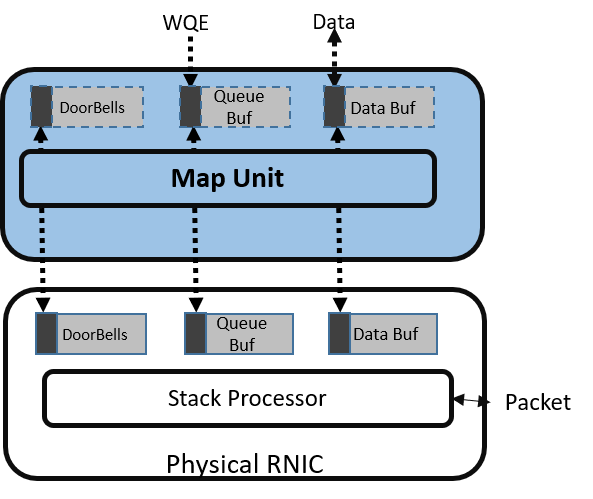
\includegraphics[width=0.9\linewidth]{images/map-unit}
	\caption{Map Unit in vRNIC}
	\label{fig:map-unit}
\end{figure}

For RDMA resources (e.g. QPs, CQs): Taking QP as an example, regularly, vRNIC record virtual RDMA resources information when the virtual QP instance are created. However, virtual QP are still not generated-associated with the RNIC. To make the mapping, the map unit will create corresponding real QP instance in RNIC based on the information of virtual QP instances, such as the same memory address information and the same device id. Equivalently, the virtual QP information are recognized in RNIC, such as QP number and QP state, and can be one-to-one synchronous with RNIC’s physical instance by lots of similar map operations in control path. All operations can be completed by calling the Verbs interface of RNIC in user space. After the mapping is completed, the work requests in the vRNIC virtual QP can be zero-copied into the RNIC. Also, data in registered memory of vRNIC can also be zero-copied to RNIC in the same way. 

For DoorBells: It needs to be mapped to the hardware doorbell in the physical NIC device space, so that vRNIC can notify the RNIC hardware processors. In vRNIC, the mapping unit will map the virtual address of the virtual doorbell to the hardware doorbell address of the corresponding physical NIC device space through a system call. As shown in Figure~\ref{fig:map-unit}, after the mapping is completed, the write operation to the vRNIC virtual doorbell is equivalent to performing the doorbell notification to the RNIC.

Map unit is the key for vRNICs' performance. Note that all mapping relationships are all one-to-one, therefore, the correctness and isolation of resources in different RDMA context are guaranteed. Meanwhile, because the mapping operation is only executed in control path, the overhead is one-off compared to data commands. For the data path, vRNICs can directly utilize the hardware processing capability of RNIC, such as DMA zero-copy and hardware protocol stack processing.

\subsection{Unified vRNIC Driver}
vRNIC is virtual device with complete RDMA attributes. However, vRNICs are still independent software in host user space. Thus, for VMs and containers, the driver (or library in containers) for vRNICs should be designed. Unification is necessary for vRNIC driver, because it hides the difference of applications' environments and makes the centralized management (e.g. the virtual layer in later section) easier.

For containers, vRNICs can be directly provided to RDMA applications in containers with some modification in containers' verbs library. However, vRNICs  and VMs' application are isolated with the hypervisor and guest OS. vRNICs needs to be recognized by VMs' hypervisor and then provided by guest OS. Thus, the I/O virtualization should be used to extend each vRNIC for VMs. Then, specific driver for vRNICs installed in guest OS. 

However, the main challenge of above is how to make vRNICs unified to all RDMA applications. Thus, the communication between vRNIC to VMs or containers must be consistent. To make vRNICs communication consistent, we design a unified protocol from vRNIC to VMs' hypervisor or containers' applications. Note that both containers' applications and VMs are processes for host. Thus, I/O channel between vRNIC and VM is shared memory with specific protocol, e.g. vhost-user. And that is nature to containers' applications. Besides, the notification is used in event descriptor.

The goal of the device driver is to support I/O process inside each guest. As shown in in Figure~\ref{fig:vrnic-driver},  the commands of RDMA application be forwarded into the memory-shared queue, and trigger events to notify the vRNIC to process them; similarly, the device driver receives interrupt notifications and reads the result from vRNIC. In short, the device driver can be implemented by a lightweight kernel module.

\begin{figure}[!ht]
\centering
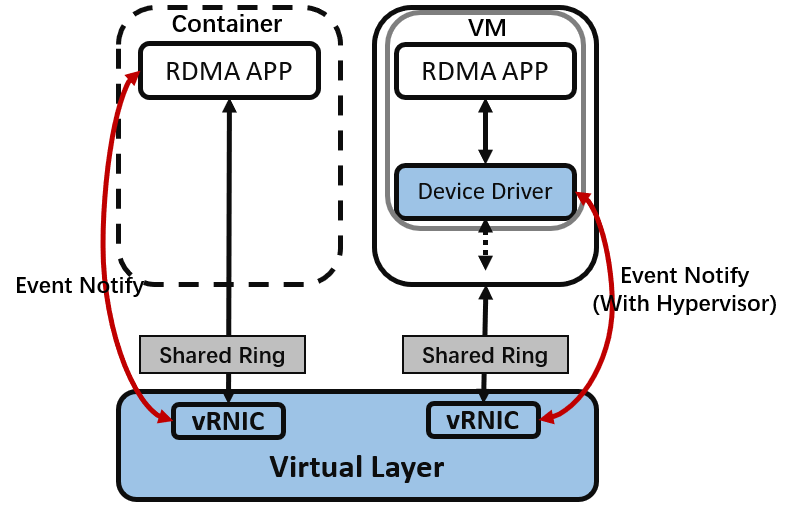
\includegraphics[width=1.0\linewidth]{images/interface-general}
\caption{Unified vRNIC Driver}
\label{fig:vrnic-driver}
\end{figure}

	
\subsection{Performance Optimization}
Trough vRNIC driver, all commands of RDMA applications can be executed in vRNICs. However, in data path of vRNIC, there is still data-copy. Also, the data commands are forwarded to vRNIC for execution. These brings the data-copy or context-switch latency for RDMA applications. 

To address above performance problems, we map RDMA resources between vRNICs and appications. However, there are two different RDMA resources for vRNICs: resources in host physical memory (such as QPs, MRs), resources in physhical RNIC (e.g. DoorBell registers). 

(1) For QPs or MRs: The fact of zero-copy is that both processes have common available physical memory pages. Same as native RDMA, the zero-copy contents are including the RDMA work request in QPs and data in MRs. 
Similar as the above I/O channels, we use shared memory to map applications' memroy to vRNICs' RDMA resources (e.g. QPs and MRs). And this mapping is feasible for both VMs and containers.

\begin{figure}[!ht]
	\centering
	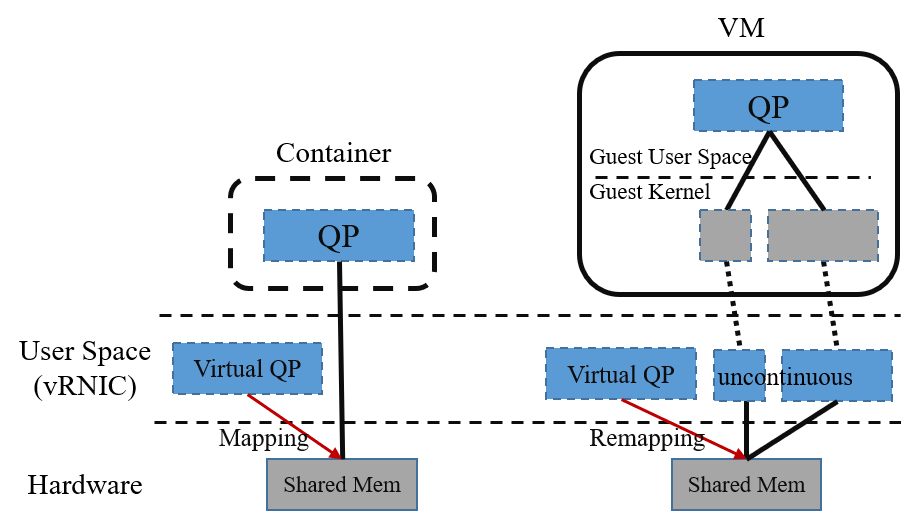
\includegraphics[width=1.0\linewidth]{images/zero-copy}
	\caption{Mapping QP to vRNIC}
	\label{fig:zero-copy}
\end{figure}

However, in the virtual machine, due to the memory management mechanism of guest operating system, the virtual machine's physical memory of the RDMA resource may be not continuous, and the mapped memory area in vRNIC is not continuous like Figure~\ref{fig:zero-copy}. So, vRNIC cannot map the virtual memory area as a virtual RDMA resource to RNIC. To solve this problem, the virtual memory remapping mechanism in user space is used. It remaps the discontinuous RDMA resource virtual memory area in vRNIC to the a block of continuous virtual memory, and the sequence of mapped physical memory page must be unchanged.

(2) For doorbells: Pressing the doorbell is necessary in RDMA data path to drive RNIC. In vRNIC, the doorbell that is mapped to physical RNIC, still need to be mapped to RDMA application to meet bypassing. Otherwise, the pressing command needs be forward to vRNIC and that’s imports apparent latency in data path.

However, the RDMA application and the vRNIC belong to two different processes on the host, and they have isolated virtual address spaces. At the same time, the doorbell register is in the device address space and cannot be mapped by shared memory. The key to solving this problem is that the process of RDMA application needs to know the physical address of the doorbell register.

\begin{figure}[!ht]
	\centering
	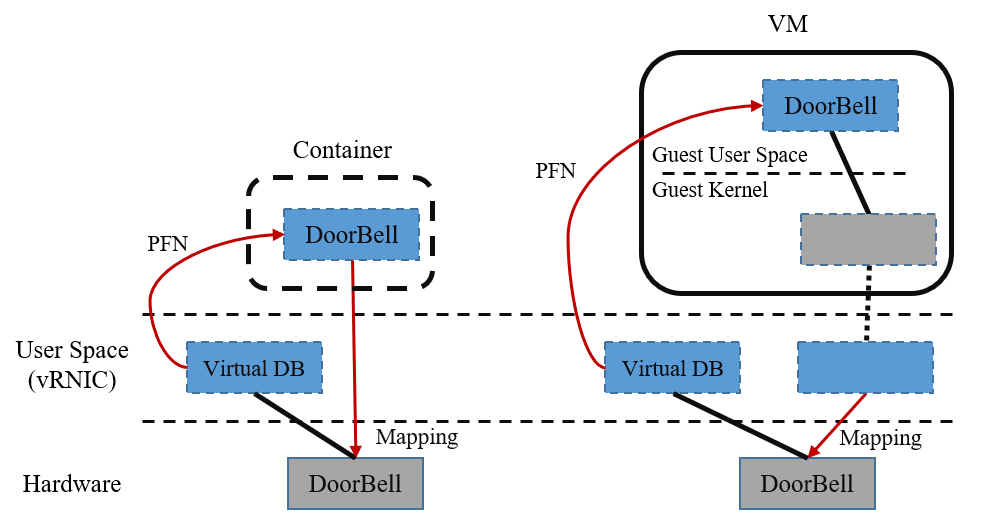
\includegraphics[width=1.0\linewidth]{images/by-pass}
	\caption{Mapping DB from vRNIC}
	\label{fig:by-pass}
\end{figure}

Therefore, when an RDMA application creates a RDMA context, as shown in Figure~\ref{fig:by-pass}, it sends a request to the vRNIC at first. Under the supervision of virtual layer, vRNIC forwarded to application with the corresponding physical address of the doorbell, commonly the physical page number. After that, the application maps its doorbell virtual address to the physical page in its own process, that needs the host kernel and hypervisor if the application in virtual machines.

